\chapter{Analiza wybranych wydajnych baz nierelacyjnych}

W rozdziale tym zostały przeanalizowane wybrane bazy nierelacyjne: Apache Cassandra\footnote{Strona główna projektu Apache Cassandra \url{http://cassandra.apache.org}} i~MongoDB\footnote{Strona główna projektu MongoDB \url{https://www.mongodb.com}}.
Opisowi został poddany model danych, architektura systemu, biblioteki klienckie oraz możliwości indeksowania i wyszukiwania pełnotekstowego. 

Niniejsza praca skupiła się na tych dwóch projektach, ponieważ reprezentują dwa różne podejścia do przechowywania danych. 
Oba są rozwiązaniami dojrzałymi, sprawdzonymi produkcyjnie przez wiele renomowanych firm, takie jak: Google, Facebook, Nokia i Netflix \cite{MongoCustomers}\cite{CassandraNetflix}.
Cieszą się dużą popularnością wśród rozwiązań NoSQL oraz wsparciem skupionych wokół nich społeczności.

\section{Kolumnowa baza Apache Cassandra}

Apache Cassandra jest wysoce skalowalną i wydajną, rozproszoną bazą kolumnową.
Została napisana w języku Java w 2008 roku przez inżynierów firmy Facebook \cite{CassandraOrigins}.
Po udanym starcie i~zyskaniu popularności została udostępniona szerokie społeczności przez Apache Incubator.
W~chwili obecnej Cassandra jest jedną z najbardziej wydajnych baz kolumnowych NoSQL przy zachowaniu pełnej skalowalności na sprzęcie dowolnej klasy.

Łączy w sobie cechy dwóch najważniejszych baz danych NoSQL, z punktu widzenia wkładu w rozwój tego zagadnienia: \textit{Google BigTable} oraz \textit{Amazon Dynamo}.
Model danych tego systemu opiera się w dużej mierze na podejściu zaproponowanym przez Google BigTable.
Bazuje on na podziale danych na tabele zawierające klucz i wartość.
Sposób funkcjonowania w środowisku rozproszonym został natomiast zaczerpnięty z Amazon Dynamo.

Baza ta została zaprojektowana tak, aby pokryć wszystkie obszary wymagań niefunkcjonalnych.
Do głównych cech systemu należą:
\begin{itemize}
    \item skalowalność horyzontalna, dzięki której dodanie kolejnego węzła zwiększa przepustowość zarówno odczytu jak i zapisu bez niedostępności dla aplikacji,
    \item replikacja i związane z nią bezpieczeństwo przed utratą danych,
    \item brak pojedynczego punktu podatności na awarie (ang. \textit{single point of failure}),
    \item dodatkowa warstwa abstrakcji w postaci języka CQL (\textit{Cassandra Query Language}).
\end{itemize}

\subsection{Model danych w bazach kolumnowych}

Apache Cassandra wprowadza następujące pojęcia zawiązane z modelem danych \cite{cassandraArchitecture}:
\begin{itemize}
    \item \textbf{kolumna}: krotka (\textit{nazwa, wartość}) wraz ze znacznikiem czasu ustalanym przez klienta,
    \item \textbf{wiersz}: posortowany zbiór kolumn będący atrybutami jednej encji, identyfikowanej przez klucz wiersza,
    \item \textbf{grupa kolumn} (ang. \textit{column family}) zwana też \textbf{tabelą}: posortowany zbiór wierszy; jest to właściwie dwuwymiarową mapą przedstawioną na rysunku \ref{fig:cassandraColumnFamily}.
    \item \textbf{przestrzeń kluczy} (ang. \textit{keyspace}): zbiór grup kolumn (tabel) dzielących wspólną strategię rozmieszczenia replik danych wśród węzłów klastra. Tworzy również przestrzeń nazw dla tabel i jest porównywana do schematu w relacyjnych bazach danych.
\end{itemize}

\begin{figure}[!ht]
\centering
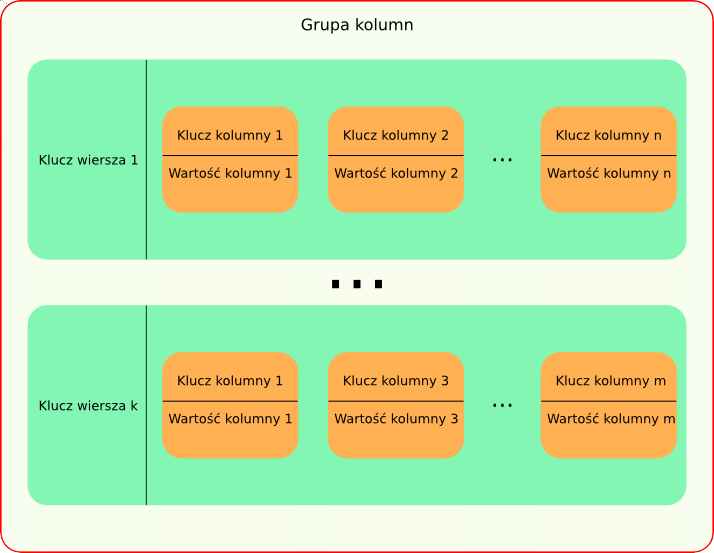
\includegraphics[width=0.7\textwidth]{figures/casModel1.png}
\caption{Schemat grupy kolumn w systemie Apache Cassandra}
\label{fig:cassandraColumnFamily}
\end{figure}

Warto wspomnieć jeszcze, że każda kolumna oprócz nazwy i wartości przechowuje znacznik czasowy (ang. \textit{timestamp}), oznaczający datę ostatniej jej modyfikacji.
Wartość ta nie jest dostarczana przez bazę danych, lecz przez klienta wraz z żądaniem zapisu danych.
Niestety nie ma możliwości wykonywania zapytań według kryterium tego znacznika czasowego, ponieważ jest wykorzystywany jedynie do rozwiązywania konfliktów do których może dojść po stronie serwera.

Dodatkowe pojęcia łączące model danych z architekturą bazy danych to:
\begin{itemize}
    \item \textbf{węzeł} (ang. \textit{node}) -- maszyna z działającym na niej serwerem Cassandry.
    Podstawowa jednostka infrastruktury.
    \item \textbf{centrum danych} (ang. \textit{datacenter}) -- zbiór węzłów w ramach, których następuje replikacja danych z przestrzeni kluczy z określonym współczynnikiem replikacji.
    Pojedyncza przestrzeń kluczy może posiadać różne współczynniki replikacji dla różnych centrów danych.
\end{itemize}

\subsection{Rola kluczy głównych w tabelach}

Bardzo ważną rolę w projektowaniu modelu danych w bazie Apache Cassandra odgrywają klucze główne tabel.
Jeżeli chcemy przeszukiwać tabelę według kryterium obejmującego jakąś kolumnę to musi być ona włączona do klucza głównego.
Podyktowane jest to względami wydajnościowymi.
Przeszukiwanie rozproszonego zbioru danych mogłoby spowodować długie oczekiwanie na odpowiedź.
Poprawne zdefiniowanie kluczy głównych jest jedną z najważniejszych kwestii podczas projektowania modelu danych w tym systemie.

Klucze główne w tabelach można podzielić na:
\begin{itemize}
\begin{samepage}
    \item \textbf{proste} -- klucze składające się pojedynczej kolumny, która jednocześnie pełni rolę klucza partycjonującego, dystrybuującego dane między węzłami sieci.
\end{samepage}

    \item \textbf{złożone} -- klucze składające się z więcej niż jednej kolumny. 
    Podczas definicji takiego klucza należy wyznaczyć kolumny należące do klucza partycjonującego (domyślnie pierwsza kolumna w definicji klucza głównego).
    Pozostałe kolumny, nieuwzględnione w tym kluczu, będą definiować kolejność sortowania wierszy w ramach jednej partycji danych.
\end{itemize}

\subsection{Zapis danych}

\subsubsection{Commit log}

Węzeł otrzymując żądanie zapisu danych najpierw zapisuje je sekwencyjnie do przechowywanego lokalnie na dysku dziennika (ang.~\textit{commit log}).
Pełni on rolę kopii zapasowej i mechanizmu optymalizacji zapisu historii przeprowadzonych operacji na wypadek awarii.
Po restarcie uszkodzonego węzła na jego podstawie węzeł jest wstanie powrócić do stanu sprzed awarii.
Zapis operacji do tego dziennika stanowi warunek konieczny do uznania jej za poprawną.
Poprzez sekwencyjny zapis operacje na danych w Cassandrze są bardzo szybkie -- nie trzeba szukać pozycji, gdzie dane mają być zapisane.

Cassandra może dokonywać synchronizacji pamięci podręcznej, reprezentującej ostatnie zmiany w~dzienniku, w dwóch trybach:
\begin{itemize}
    \item \textbf{okresowym} -- zapisy są natychmiastowo potwierdzane, a dziennik jest po prostu zsynchronizowany z określoną w konfiguracji częstotliwością.
    \item \textbf{wsadowym} -- zapis nie zostanie potwierdzony, zanim dane z dziennika nie zostaną zapisane do pliku dziennika na dysku. 
    W celu uniknięcia dostępu do dysku przy każdym żądaniu, Cassandra oczekuje na kolejne żądania zapisu, aby wykonać je wsadowo. 
    Maksymalny czas oczekiwania określony przez jeden z parametrów konfiguracji.
\end{itemize}
Wybór pomiędzy tymi dwoma trybami daje wybór użytkownikowi między pewnością zapisu a~szybkością odpowiedzi. Domyślnym trybem jest tryb wsadowy.

\subsubsection{Memtables}

Po zapisie do commitlogu Cassandra synchronizuje dane do struktur zwanych \textit{memtables}.
Jest to bufor przechowywany w pamięci operacyjnej, w którym zapisane są wartości kolumn wraz kluczami.
Na jedną tabelę przypada jedna aktywna struktura memtable.
Ostatecznie, jest ona zapisywana na dysku.
Zapis jest wyzwalany w momencie, gdy:
\begin{itemize}
\begin{samepage}
    \item ich rozmiar przekroczy konfigurowalny limit,
\end{samepage}
    \item commitlog zbliża się do swojego maksymalnego rozmiaru i wymusza zrzut struktur memtables w celu zwolnienia segmentu commitlogu.
    \item upłynie czas określony w konfiguracji systemu.
\end{itemize}

\subsubsection{SSTables}

Struktury memtable są zapisywane na dysku do struktur danych zwanych SSTables (ang.~\textit{Sorted Strings Tables}).
SSTables są plikami, w których Cassandra przechowuje fizycznie swoje dane.
Raz zapisane SSTable nie może zostać zmienione.
Pliki te są łączone (ang. \textit{compaction}) po przekroczeniu zapisanego w konfiguracji limitu nowo zapisanych plików.
Ma to zapobiec nadmiernemu przeszukiwaniu wielu plików podczas odczytów.
W skład plików zapisywanych na dysku wchodzą pliki danych, pliki indeksów i pliki filtru Blooma, którego działanie zostało przybliżone w~sekcji~\ref{sec:cassandraBloomFilter}.

Warte uwagi jest to, że w kontraście do baz relacyjnych, zarówno zapis do commitlogu jak i~do SSTable nie zmienia już istniejących plików, w związku z tym nie wymaga przeszukiwania i~odczytu danych z dysku.
To z kolei przekłada się na teoretycznie bardzo szybkie operacje zapisu Cassandry.

\subsection{Odczyt danych}

W pierwszej kolejności na żądanie odczytu Cassandra sprawdza, czy oczekiwana wartość nie znajduje się w przechowywanej w pamięci strukturze memtable.
Jeśli oczekiwana wartość nie została odnaleziona w memtable, oznacza to konieczność dostępu do SSTable na dysku.
Zanim jednak zostanie przeszukany indeks to Cassandra sprawdza przy pomocy filtru Blooma, czy szukana wartość w ogóle przynależy do zbioru. 
Jeśli odpowiedź jest negatywna to Cassandra nie przystępuje do przeszukiwania indeksu.
Po otrzymaniu pozytywnej odpowiedzi następuje binarne przeszukiwanie posortowanego indeksu.
Wszystkie te kroki mają na celu jak najszybszą odpowiedź dla klienta.

\subsubsection{Filtr Blooma} \label{sec:cassandraBloomFilter}

Filtr Blooma jest kluczowym elementem decydującym czy baza ma w~ogóle przystępować do przeszukiwania indeksu w poszukiwaniu szukanego klucza.
Każda SSTable posiada własny filtr.
Jest to probabilistyczna struktura danych stworzona w~1970~roku przez Burtona Blooma.
Jest używana do reprezentacji zbioru elementów pozwalającej na szybkie określenie przynależności elementu do zbioru z zadanym podczas jej tworzenia prawdopodobieństwem.

Omawiana struktura danych jest $m$-bitową tablicą.
Korzysta z $k$ niezależnych funkcji skrótu odwzorowujących elementy reprezentowanego zbioru na jedną z pozycji wynikowej tablicy.
Po wypełnieniu w ten sposób tablicy sprawdzenie czy zadanego elementu nie ma w zbiorze polega na sprawdzeniu, czy którakolwiek z funkcji wskazuje na zero w tablicy.

Filtr posiada następujące właściwości:
\begin{itemize}
    \item zużywa stałą ilość pamięci,
    \item koszt wstawienia i zapytanie jest stały: $O(k)$,
    \item złożoność obliczeniowa zapytania nie zależy od $m$,
    \item obliczanie $k$ niezależnych funkcji skrótu można realizować równolegle.
\end{itemize}

Oprócz pewnego określenia, że zadany element nie należy do zbioru filtr może skłamać zwracając wartość pozytywną (sytuacja określana jako \textit{false positive}).
Prawdopodobieństwo  błędnego  przypuszczenia  przynależności  elementu do zbioru $n$-elementowego jest wyrażane przez wzór \ref{eq:fpProp}.
Szansa błędu rośnie wraz z liczbą wstawianych elementów $n$ i maleje wraz ze wzrostem rozmiaru tablicy bitowej $m$.

\begin{equation} \label{eq:fpProp}
    P_{fp} = \left(1 - \left(1 - \frac{1}{m}\right)^{kn}\right)^k
\end{equation}

Dzięki niemu można wyznaczyć optymalną długość tablicy $m$ (wzór \ref{eq:tabSize}) oraz liczbę funkcji skrótu $k$ (wzór \ref{eq:funCount}) dla oczekiwanego prawdopodobieństwa błędu $P_{fp}$ i $n$ elementów w~zbiorze~\cite{BloomFilter}.

\begin{equation} \label{eq:tabSize}
    m = \frac{-n \cdot \ln{\left(P_{fp}\right)}}{\ln{(2)}^2}
\end{equation}

\begin{equation} \label{eq:funCount}
    k = \frac{m}{n} \cdot \ln{\left(2\right)}
\end{equation}

W bazie danych Apache Cassandra jest możliwość konfiguracji współczynnika prawdopodobieństwa \textit{false positive} dla filtru Blooma.
Dokonuje się tego per tabela ustawiając parametr \textit{bloom\_filter\_fp\_chance} \cite{cassandraBloomConf}. 

\subsection{Rozproszona architektura systemu}

Ze względu na implementacje w oparciu o język Java, Cassandra jest w pełni przenośna pomiędzy różnymi systemami operacyjnymi. 
Głównym celem jej jest obsługa dużych obciążeń danych w wielu węzłach bez pojedynczego punktu awarii.
Dokonuje tego dzięki rozproszonej architekturze peer-to-peer, gdzie dane są rozdystrybuowane pomiędzy węzły systemu.

Cechami tej rozproszonej architektury są:
\begin{itemize}
\begin{samepage}
    \item Wszystkie węzły w klastrze mają tą samą rolę. Każdy z nich jest niezależny i jednocześnie połączony z pozostałymi.
\end{samepage}
    \item Każdy węzeł w klastrze może przyjmować żądania odczytu i zapisu niezależnie od tego, gdzie dane faktycznie znajdują się w klastrze.
    \item Kiedy węzeł przestaje działać, żądania odczytu/zapisu mogą być obsługiwane przez inne węzły w sieci.
\end{itemize}

\subsubsection{Komunikacja wewnętrzna}

Protokół \textit{gossip} \cite{cassandraGossipProtocol} jest protokołem komunikacji peer-to-peer, za pomocą którego węzły okresowo wymieniają między sobą informacje o stanie własnym i innych węzłów, o których mają informację. 
Proces ten przebiega co sekundę i wymienia komunikaty z maksymalnie trzema innymi węzłami w~klastrze.
Węzły wymieniając informacje o sobie i innych węzłach, o których posiadają informację, bardzo szybko doprowadzają do sytuacji, w której każdy węzeł zna stan wszystkich pozostałych węzłów w klastrze.
Każda wymieniona wiadomość kontrolna ma przypisaną wersję, tak że podczas ich wymiany starsze informacje są nadpisywane najbardziej aktualnym stanem dla danego węzła. 

Podczas pierwszego uruchamiania klastra ważne jest, aby każdy węzeł posiadał listę węzłów początkowych (ang. \textit{seed nodes}), które przechowują adresy wszystkich węzłów w klastrze.
Podczas pierwszego cyklu wymiany informacji między węzłami, węzły te inicjują cały proces.
Domyślnie węzeł zapamiętuje inne węzły, z którymi plotkuje pomiędzy kolejnymi cyklami.
Rola węzła początkowego nie ma celu innego niż inicjowanie procesu wymiany informacji dla nowych węzłów dołączających do klastra.

\subsubsection{Wykrywanie awarii}

Wykrywanie awarii polega na określaniu z otrzymanych wiadomości (\textit{gossips}) o stanie i ich historii, czy inny węzeł w sieci nie odpowiada, lub rozpoczął ponownie odpowiadać na zapytania po powrocie z awarii.
Cassandra może także uniknąć wysyłania żądań do węzłów, które są dostępne, ale działają pod dużym obciążeniem.

Proces wymiany informacji o stanie pozwala na śledzenie stanu innych węzłów bezpośrednio lub pośrednio -- bazując na informacjach z drugiej ręki.
Zamiast ustalonego progu do oznaczania niesprawnych węzłów, Cassandra wykorzystuje mechanizm przyrostowego wykrywania awarii, aby obliczyć oddzielny próg dla każdego węzła biorąc pod uwagę wydajność sieci, obciążenie pracą i warunki historyczne.
Konfigurując odpowiedni parametr systemu można dostosowywać czułość detektora awarii.

Awaria węzła może wynikać z różnych przyczyn, takich jak awaria sprzętu i przerwy w dostępie do sieci.
Przestoje w pracy są często przejściowe, ale mogą trwać też przez dłuższy czas.
Inne węzły będą periodycznie próbowały odnowić łączność z nieosiągalnymi węzłami, aby sprawdzić czy są dostępne z powrotem.
W celu trwałej zmiany przynależności węzła do klastra, administrator musi go jawnie dodać lub usunąć posługując się dostarczanym przez Cassandrę narzędziem do zarządzania węzłami.

\subsection{Dystrybucja i replikacja danych}

W rozproszonej architekturze Cassandry dystrybucja i replikacja danych idą w parze.
Dane są uporządkowane według tabeli i identyfikowane przez klucz główny, który określa, w którym węźle dane są przechowywane.
Repliki są kopiami wierszy.

Czynniki wpływające na replikację obejmują: 
\begin{itemize}
\begin{samepage}
    \item \textbf{Wirtualne węzły}: określają przydzielenie danych do fizycznej maszyny.
\end{samepage}
    \item \textbf{Moduł partycjonujący}: dzieli dane w klastrze.
    \item \textbf{Strategia replikacji}: określa repliki dla każdego wiersza danych.
\end{itemize}

\subsubsection{Spójne haszowanie}

Spójne haszowanie (ang.~\textit{consistent hashing}) jest algorytmem pozwalającym na organizację danych w klastrze w rodzaj pierścienia i przypisywanie odpowiednim węzłom odpowiedzialności za poszczególne fragmenty tego pierścienia. 
Prostym sposobem organizacji danych w pierścień jest przypisanie ich kluczom wartości funkcji skrótu z pewnego zakresu $\left[0, MAX\right]$ \cite{consistentHashing}.

Najprostszy wariant rozłożenia danych pomiędzy węzły przedstawia Rysunek \ref{fig:cassandraConsistenHashing}.
Cztery węzły dzielą między sobą odpowiedzialność za odpowiednie partycje danych, które są podzielone według wyniku funkcji skrótu przyjmującej jako argument klucz główny.
Kolor węzła odpowiada kolorowi fragmentu pierścienia danych, za który odpowiada.

\begin{figure}[!ht]
\centering
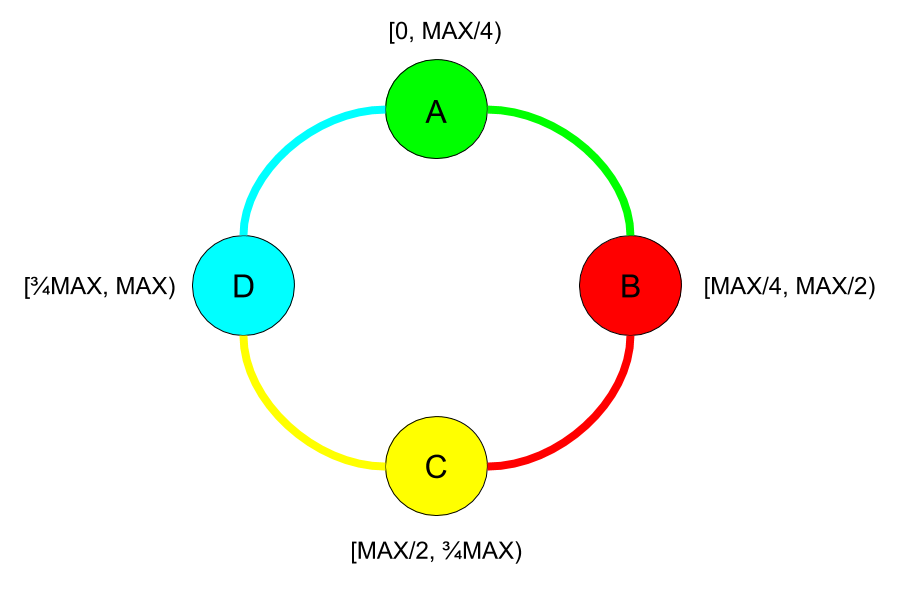
\includegraphics[width=0.7\textwidth]{figures/consisten_hashing.png}
\caption{Pierścień danych i ich podział pomiędzy węzły w algorytmie \textit{Consistent hashing}}
\label{fig:cassandraConsistenHashing}
\end{figure}

\subsubsection{Wirtualne węzły}

Przydzielanie odpowiedzialności za jedną, dużą partycję poszczególnym węzłom, sprawia, że wszelkie reorganizacje węzła są kłopotliwe i znacząco obciążające.
Sposobem zmniejszenia tych niedogodności jest podział fizycznie istniejącej maszyny na węzły wirtualne (ang.~\textit{vnodes}), który został wprowadzony w wersji 1.2 Cassandry.
Dzielą one dużą partycję przydzieloną fizycznej maszynie na mniejsze części.
Odpowiedzialność za te części może być później przekazana do innych węzłów jak zajdzie taka potrzeba.
Dzieje się to w~sposób całkowicie automatyczny i~domyślna liczba wirtualnych węzłów działających na jednym węźle fizycznym to 256 \cite{virtualNodes}.
Podział partycji na mniejsze ułatwia to wiele zadań w systemie:
\begin{itemize}
    \item Ponowne równoważenie klastra, gdy jest dodawany lub usuwany węzeł.
    Dodany węzeł podejmuje odpowiedzialność za równą porcję danych z pozostałych węzłów w klastrze.
    Jeśli węzeł popsuje się to obciążenie jest równomiernie dystrybuowane na inne węzły.
    \item Odbudowywanie martwych węzłów jest szybsze, ponieważ angażuje pozostałe węzły w klastrze.
\end{itemize}

\subsubsection{Replikacja danych}

Cassandra przechowuje repliki na wielu węzłach, aby zapewnić niezawodność i odporność na awarie.
Strategia replikacji określa węzły, w których są umieszczane kopie.
Całkowita liczba replik w klastrze jest określana jako współczynnik replikacji.
Współczynnik replikacji wynoszący~1 oznacza, że istnieje tylko jedna kopia każdego wiersza w klastrze.
Jeśli węzeł przechowujący wiersz ulegnie awarii to tego wiersza już nie da się odzyskać.
Współczynnik replikacji równy~2 określa dwie kopie tego samego wiersza, każda przechowywana na innym węźle.
Wszystkie kopie są równie ważne -- nie istnieje główna lub nadrzędna kopia.
Zasadą jest, że współczynnik replikacji nie powinien przekraczać liczby węzłów w klastrze.
Można jednak go zwiększyć, a~następnie dodać później wymaganą liczbę węzłów \cite{cassandraDataReplication}.

Dostępne są dwie strategie replikacji:
\begin{itemize}
\begin{samepage}
    \item \textbf{Prosta strategia} (ang. \textit{Simple Strategy}): używana wyłącznie w topologiach zawierających pojedyncze centrum danych w klastrze.
    Repliki danych są rozmieszczane na kolejnych węzłach klastra bez uwzględniania podziału na centra danych.
\end{samepage}
    \item \textbf{Strategia topologii sieciowej} (ang. \textit{Network Topology Strategy}): używana w klastrach z~wieloma centrami danych.
    Określa jak wiele replik przestrzeni kluczy powinno być rozmieszczonych w poszczególnych centrach danych.
\end{itemize}

Strategia replikacji jest definiowana dla przestrzeni kluczy i jest ustawiana podczas jej tworzenia.

\subsection{Biblioteki klienckie i narzędzia dostępowe}

Apache Cassandra dzięki szerokiemu wsparciu społeczności posiada bogatą kolekcję narzędzi dostępowych. 
Znajdziemy w niej biblioteki na większość najpopularniejszych języków wysokopoziomowych, dzięki którym istnieje możliwość łatwego oraz szybkiego łączenia się z bazą danych w aplikacjach napisanych w językach Java, Python, C\#, Ruby, PHP.

Pierwszym oraz najważniejszym ze względów historycznych, sposobem łączenia się z bazą danych Cassandra jest \textit{Thrift API}.
Biblioteka ta służy do zdalnego wywoływania procedur między programami napisanymi w różnych językach, takich jak C++, Java, Erlang lub JavaScript.
Na jej potrzeby stworzony został pewien metajęzyk opisujący serwisy oraz dane wymieniane pomiędzy uczestnikami protokołu.

Nowsze biblioteki klienckie odeszły od tego sposobu dostępu do bazy danych na rzecz języka \textit{CQL} (ang.~\textit{Cassandra Query Language}), który jest bardzo podobny do SQL.

\subsubsection{CQL}

CQL jest to imperatywny język programowania, oparty w dużej mierze na języku SQL.
Umożliwia on modyfikację struktury bazy danych, jak i również operacje na danych.
Posiada on wiele elementów znanych z SQL, jak np. polecenia SELECT, INSERT, UPDATE, DELETE.
Ich zastosowanie nie różni się od ich odpowiednika z baz relacyjnych. 
Ze względu na specyfikę modelu danych w Cassandrze CQL nie posiada operacji złączeń.
W zakresie manipulacji danymi (DML -- \textit{Data Manipulation Language}) można przyjąć, że CQL jest niepełnym dialektem języka SQL.

Różnicą pomiędzy CQL a SQL jest część odpowiedzialna za manipulację strukturami danych (DDL -- \textit{Data Definition Language}).
W bazie danych Cassandra nie istnieją struktury znane z~baz relacyjnych, dlatego jest brak odpowiadających im poleceń.
Zamiast tego istnieją polecenia pozwalające na tworzenie przestrzeni kluczy i rodzin kolumn.

\subsection{Wsparcie dla wyszukiwania pełnotekstowego}

Cassandra posiada nieoficjalne wsparcie dla wyszukiwania pełnotekstowego w postaci rozszerzenia jakim jest \textit{Elassandra}\footnote{Strona główna projektu Elassandra \url{https://www.elassandra.io/}}.
Elassandra ściśle integruje silnik wyszukiwania pełnotekstowego \textit{Elasticsearch} z bazą danych Cassandra osadzając jego odpowiednio zmodyfikowany kod w każdym węźle Cassandry.
Elasticsearch tworzy indeks wtórny na potrzeby wyszukiwania tekstowego.
Dodatkowo udostępnia RESTful API w celu komunikacji z aplikacjami klienckimi. 
Rola Cassandry sprowadza się do magazynu danych i konfiguracji \cite{elassandraArchitecture}.
W przejrzysty sposób ilustruje to rysunek~\ref{fig:elassandraSchema}.
Tabela \ref{tab:ElassandraMappings} przedstawia podstawowe pojęcia związane z Cassandrą i ich odpowiedniki w Elasticsearch.

\begin{figure}[!ht]
\centering
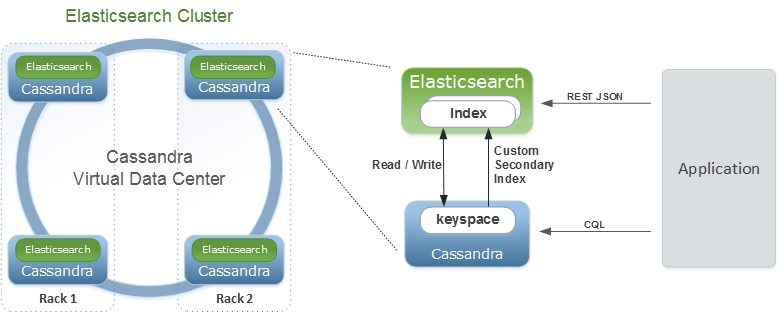
\includegraphics[width=0.8\textwidth]{figures/elassandra1.jpg}
\caption{Schemat integracji wtyczki Elasticsearch z bazą danych Cassandra \cite{ElassandraRepo}}
\label{fig:elassandraSchema}
\end{figure}

\begin{table}[!ht]
\centering
\caption{Podstawowe pojęcia związane z Cassandrą i ich odpowiedniki w Elasticsearch}
\begin{tabular}{|l|l|l|}
\hline
\textbf{Cassandra} & \textbf{Elasticsearch} & \textbf{Opis} \\ \hline
Centrum danych & Klaster & \begin{tabular}[c]{@{}l@{}}Wszystkie węzły centrum danych \\ tworzą klaster Elasticsearch\end{tabular} \\ \hline
Węzeł & Węzeł & \begin{tabular}[c]{@{}l@{}}Każdy węzeł Cassandry jest \\ węzłem Elasticsearch\end{tabular} \\ \hline
Przestrzeń kluczy & Indeks & \begin{tabular}[c]{@{}l@{}}Indeks jest mapowany na \\ pojedynczą przestrzeń kluczy \\ w Cassandrze\end{tabular} \\ \hline
Tabela & Typ & \begin{tabular}[c]{@{}l@{}}Każdy typ dokumentu Elasticsearch \\ jest mapowany przez tabelę\end{tabular} \\ \hline
Wiersz & Dokument & \begin{tabular}[c]{@{}l@{}}Dokumentowi odpowiada jeden \\ wiersz w tabeli\end{tabular} \\ \hline
Komórka & Pole & \begin{tabular}[c]{@{}l@{}}Pole dokumentu jest przekładane \\ na komórkę w wierszu tabeli\end{tabular} \\ \hline
\begin{tabular}[c]{@{}l@{}}Złożony typ \\ zdefiniowany \\ przez użytkownika\end{tabular} & \begin{tabular}[c]{@{}l@{}}Obiekt lub \\ pole zagnieżdżone\end{tabular} & \begin{tabular}[c]{@{}l@{}}W celu przechowywania obiektów \\ Elasticsearch tworzone są złożone\\ typy kolumn\end{tabular} \\ \hline
\end{tabular}
\label{tab:ElassandraMappings}
\end{table}

\section{Dokumentowa baza MongoDB}

\textit{MongoDB} jest bazą nierelacyjną typu dokumentowego.
Dane są zorganizowane w postaci elastycznych dokumentów zapisywanych w formacie pochodnym do JSON o nazwie \textit{BSON}.
Jest on formatem serializacji dokumentów w formacie JSON to postaci binarnej w celu zapisu na dysku lub transportu przez sieć \cite{BSONSpecification}.
Istnieje również pojęcie kolekcji dokumentów, jednak spójność struktury dokumentów w obrębie jednej kolekcji nie jest wymagana.

System ten posiada mechanizmy modyfikacji wartości pojedynczych atrybutów.
Zmiany te są atomowe, to znaczy, że wykonywane się wszystkie operacje lub żadna, a system wraca do stanu początkowego.
Jest to namiastka systemu transakcyjności znanego z relacyjnych baz danych.
Omawiana baza danych posiada również wsparcie dla operacji \textit{Map/Reduce}. 
MongoDB jest rozproszoną bazą danych, więc wysoka dostępność, skalowanie horyzontalne i dystrybucja danych są wbudowane i łatwe w użyciu.

Jedną z funkcjonalności, która wyróżnia MongoDB na tle innych baz NoSQL, takich jak Cassandra, jest możliwość przechowywania w niej dużych plików.
Odbywa się to przy zastosowaniu specjalnego systemu zapisu \textit{GridFS} \cite{GridFSManual}.
Dzięki jego wykorzystaniu możliwe jest przechowywanie plików, tak samo jak przechowywane są dokumenty, bez spadku wydajności całego systemu bazodanowego.

Kolejnym elementem wartym uwagi, który wyróżnia się od innych systemów NoSQL jest powłoka tej aplikacji, która funkcjonuje jako interpreter języka \textit{JavaScript}.
Dzięki temu operowanie na tej bazie sprowadza się do pisania skryptów w tym języku.

\subsection{Model danych} \label{sec:MongoModelDanych}

MongoDB jest bazą danych o modelu danych opartym na dokumentach.
Dokumenty te są zapisywane we wcześniej wspomnianym formacie BSON.
Każdy z nich jest przechowywany w~jakiejś kolekcji.
Kolekcje są to zbiory dokumentów, które do pewnego stopnia powinny być ze sobą spójne pod względem zawartości, lecz nie ma odgórnego mechanizmu sprawdzającego spójność dokumentów w kolekcji.
Są one odpowiednikami tabel w relacyjnych bazach danych.

Wielkość każdego dokumentu jest ograniczona do 16 MB \cite{DocumentsManual}.
Nie jest to ograniczenie związane z implementacją tej bazy danych.
Ma ono na celu uświadomienie architektowi bazy danych, że jeśli jego projekt zakłada przechowywanie dokumentów, które są tak duże to najprawdopodobniej można go uprościć i znacznie przyspieszyć działanie całego systemu.

\subsubsection{Modelowanie relacji}

Jednym z najważniejszych elementów podczas projektowania dokumentowej bazy danych, są relacje pomiędzy obiektami.
Istnieją dwa sposoby rozwiązania tego problemu w MongoDB \cite{MongoDBRefs}:
\begin{enumerate}
    \item \textbf{Osadzenie jednego dokumentu w drugim} -- podejście to ma niewątpliwą zaletę, jest bardzo szybkie oraz proste do zaimplementowania.
    W przypadku modelowania relacji jeden do wielu zamiast pojedynczego obiektu należy zapisać ich listę.
    Problem powstaje, gdy zagnieżdżone dokumenty są w relacji z innymi encjami (relacja wiele do wielu).
    \item \textbf{Zapisywanie referencji do innego dokumentu} -- podejście znane z baz relacyjnych.
    Aplikacje korzystające z MongoDB używają jednej z dwóch metod do odwoływania się do innych dokumentów:
    \begin{itemize}
        \item \textbf{Ręczne odwołania}, gdzie zapisywane jest tylko pole \textit{\_id} innego dokumentu jako referencja.
        Aplikacja kliencka może wtedy wykonać kolejne zapytanie, aby pobrać powiązany dokument.
        Tego rodzaju referencje są proste i wystarczające w większości przypadków użycia.
        \item \textbf{Odwołanie typu \textit{DBRef}} to odwołanie przechowujące, oprócz pola \textit{\_id} powiązanego dokumentu, nazwę kolekcji gdzie jest zapisany dokument, oraz opcjonalnie nazwę bazy danych gdzie się znajduje dana kolekcja.
        Korzystając z tych wartości możliwe jest łatwiejsze powiązanie dokumentów z różnych kolekcji, a nawet baz danych.
        Analogicznie jak w przypadku pierwszego rodzaju odwołania aplikacja kliencka musi wykonać dodatkowe zapytania w celu pobrania dodatkowych informacji.
        Wiele bibliotek klienckich posiada metody pomocnicze tworzące zapytania po dokumenty, do których odwołują się referencje DBRef.
        Warto zaznaczyć, że nie robią tego automatycznie lecz tylko na żądanie.
        
        Odwołania DBRef zapewniają wspólny format i typ przedstawiania relacji między dokumentami.
        Format DBRef zapewnia również wspólną semantykę reprezentowania powiązań między dokumentami jeżeli baza danych musi współpracować z wieloma szkieletami aplikacji i narzędziami.
    \end{itemize}
\end{enumerate}

Warto odnotować, że w MongoDB w wersji 3.2 wprowadzono nową fazę agregacji o nazwie \textit{\$lookup}.
Działa podobnie do operacji lewego złączenia zewnętrznego (LEFT OUTER JOIN) znanej z relacyjnych baz danych.
Do każdego dokumentu wyjściowego zostaje dodane pole z listą dokumentów, które zostały dopasowane ze \enquote{złączonej} kolekcji.
Zmodyfikowane tak dokumenty zostają przekazane do kolejnych etapów agregacji.
Ograniczenie tej operacji polega na tym, że przeszukiwana kolekcja musi znajdować się w tej samej bazie danych, co kolekcja, na której wykonujemy operację agregacji.

\subsubsection{Indeksy}

W celu przyspieszenia wyszukiwania w bazie danych MongoDB należy wykorzystać mechanizm indeksowania pól.
Jest on analogiczny do podejścia znanego z relacyjnych baz danych.
Indeks można założyć w ramach pojedynczej kolekcji, analogicznie jak to ma miejsce w relacyjnych systemach baz danych, gdzie indeks jest zakładanych na pojedynczej tabeli.

MongoDB udostępnia wiele różnych typów indeksów do obsługi określonych typów danych i~zapytań \cite{MongoDBIndexes}:
\begin{itemize}
    \item \textbf{Indeks na pojedynczym polu}: oprócz domyślnie zdefiniowanego indeksy na polu \textit{\_id}, system ten wspiera tworzenie posortowanych indeksów na pojedynczym polu dokumentu.
    \item \textbf{Indeks złożony}: istnieje możliwość utworzenia indeksów na zestawie pól dokumentu.
    \item \textbf{Indeks typu \textit{multikey}}: używany do indeksowania zawartości przechowywanej w tablicach.
    Jeżeli użytkownik utworzy indeks na polu przechowującym tablicę, MongoDB wprowadza osobne wpisy w indeksie dla każdego elementu tablicy.
    System ten automatycznie określa, czy ma utworzyć indeks typu \textit{multikey}, sprawdzając czy indeksowane pole zawiera tablicę.
    \item \textbf{Indeks geoprzestrzenny}: specjalny typ indeksu dla danych geoprzestrzennych.
    \item \textbf{Indeks tekstowy}: wspomaga przeszukiwanie pełnotekstowe dokumentów.
    Indeks tego typu analizuje wybrane pola pod względem leksykalnym w danym języku i indeksuje z nich słowa kluczowe w podstawowej formie.
    \item \textbf{Indeks bazujący na wartości funkcji haszującej}: struktura indeksu jest tworzona z~wartości funkcji haszującej wybrane pole dokumentu.
    Te indeksy mają bardziej losowy rozkład wartości wzdłuż ich zasięgu. 
    Są wykorzystywane tylko do wyszukiwań bazujących na równości i nie wspierają kwerend opartych na zakresie.
    Pomimo to ich głównym zastosowaniem jest wspomaganie partycjonowania danych w klastrze bazując na wartości funkcji skrótu.
\end{itemize}

\subsection{Transakcyjność operacji}

W MongoDB operacje na pojedynczych dokumentach są atomowe.
Dzięki możliwości przechowywania zagnieżdżonych dokumentów i tablic do przechowywania relacji między danymi w~pojedynczym dokumencie, zamiast normalizować je w wiele dokumentów i kolekcji, atomowość operacji na pojedynczym dokumencie eliminuje potrzebę transakcji na wielu dokumentach w~wielu przypadkach użycia.

W sytuacji, gdy wymagana jest atomowość modyfikacji wielu dokumentów lub spójność między odczytami do wielu z nich, MongoDB umożliwia wykonywanie transakcji z wieloma dokumentami w zbiorze replik.
Takie transakcje można używać w celu wykonywania wielu operacji na kolekcjach, bazach danych i dokumentach.
Działają zgodnie z zasadą \enquote{wszystko albo nic}.
Kiedy transakcja zostanie zatwierdzona, wszystkie zmiany danych dokonane w transakcji zostaną zapisane.
Jeśli jakakolwiek operacja w transakcji zakończy się niepowodzeniem, zostanie ona przerwana, a wszystkie zmiany danych dokonane w transakcji zostaną odrzucone.
Do momentu zatwierdzenia żadne operacje zapisu w transakcji nie są widoczne poza nią \cite{MongoDBTransactions}.

\subsection{Podstawowe komponenty systemu}

MongoDB składa się z kilku komponentów:
\begin{itemize}
    \item \textbf{mongod} -- usługa, która odpowiada za działanie bazy danych.
    Jest uruchamiana w trybie \textit{daemon} w systemach z rodziny Unix oraz jako \textit{Windows service} w  systemie Windows.
    Jest niezbędna do działania całego systemu i zdolna do samodzielnego wykonania replikacji danych pomiędzy różnymi węzłami sieci.
    \item \textbf{mongos} -- proces uczestniczący w określaniu lokalizacji wyszukiwanych danych w rozproszonym środowisku MongoDB.
    Dzięki temu baza danych wydaje się tworem spójnym i~jednorodnym dla zewnętrznych klientów.
    \item \textbf{mongo} -- interaktywna konsola JavaScript.
    Dostarcza wszechstronny interfejs dla administratorów systemu, a także sposób dla programistów do testowania zapytań i operacji bezpośrednio na bazie danych.
\end{itemize}

\subsection{Działanie w środowisku rozproszonym}

Podobnie jak Apache Cassandra, MongoDB bardzo dobrze działa w środowisku rozproszonym.
Posiada wbudowane wsparcie dla mechanizmów partycjonowania, replikacji danych i operacji Map/Reduce.

Zbiór replik (ang.~\textit{replica set}) jest grupą instancji \textit{mongod}, które utrzymują ten sam zestaw danych.
Zawiera on kilka węzłów zawierających dane i opcjonalnie jeden węzeł arbitrażowy.
Z~węzłów zawierających dane jeden i tylko jeden jest uważany za węzeł główny, podczas gdy pozostałe są węzłami drugorzędnymi.
Replikacja danych jest w pełni asynchroniczna.
Wybór jednostki głównej spośród węzłów klastra dokonuje się w sposób automatyczny.
W momencie, gdy węzeł główny nie komunikuje się z pozostałymi członkami zbioru przez więcej niż skonfigurowany czas (parametr \textit{electionTimeoutMillis} -- domyślnie 10 sekund), jeden z drugorzędnych węzłów ogłasza \enquote{wybory} nowego głównego węzła.
W odpowiedzi klaster dokonuje wyboru nowego podstawowego węzła i wznawia normalną pracę. Rysunek \ref{fig:mongoAutoFailover} przedstawia wyżej opisanych schemat działania automatycznego przełączenia awaryjnego.

\begin{figure}[!ht]
\centering
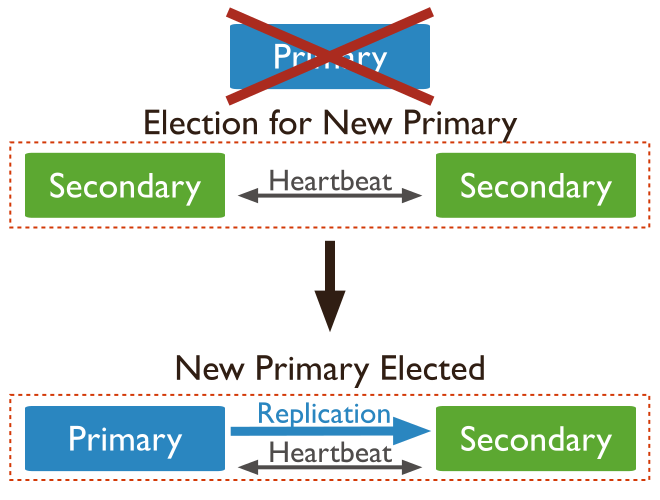
\includegraphics[width=0.6\textwidth]{figures/replica-set-trigger-election.png}
\caption{Automatyczne przełączenie głównego węzła w sytuacji awaryjnej \cite{MongoDBReplication}}
\label{fig:mongoAutoFailover}
\end{figure}

\subsection{Biblioteki klienckie i narzędzia dostępowe}

MongoDB posiada bogatą bazę oficjalnie wspieranych bibliotek klienckich.
Znajdziemy rozwiązania dostępne w praktycznie wszystkich najpopularniejszych językach programowania, począwszy od C/C++, które można osadzić w aplikacjach popularnej w dzisiejszych czas platformy \textit{Internet of Things}, po Javę i popularne języki skryptowe: Python, PHP, Ruby i JavaScript, popularyzując użycie MongoDB w aplikacjach internetowych.
Wszystkie te biblioteki komunikują się z bazą za pomocą \textit{MongoDB Wire Protocol}~\cite{MongoDBWireProtocol}, na którego żądania MongoDB nasłuchuje domyślnie na porcie TCP/IP 27017.

Istnieją też otwarte rozbudowane środowiska administracyjne dla MongoDB automatyzujące i~ułatwiające pracę administratorów.
Są to m. in.: Mongo-Express, Robo 3T (wcześniej znane jako Robomongo) oraz MongoDB Compass (w dwóch wersjach: darmowa wersja Community Edition i~bardziej rozbudowana jako część płatnego wsparcia dostępnego u twórców bazy danych).

\subsection{Wyszukiwanie pełnotekstowe}

MongoDB wspiera wyszukiwanie pełnotekstowe.
Aby móc wykonywać tego typu zapytania należy utworzyć indeks tekstowy na wybranych polach dokumentów, które chcemy przeszukiwać, a w zapytaniu należy użyć operatora \textit{\$text}.
Na jedną kolekcję może przypadać maksymalnie jeden indeks tekstowy, ale taki indeks może obejmować wiele pól.

Operator \textit{\$text} dzieli zadany ciąg znaków do wyszukania używając białych znaków i większości znaków interpunkcyjnych jako separatorów.
Zwracane są dokumenty, które zostały dopasowane do któregokolwiek z zadanych tokenów.
Przykładowo, można użyć zapytania przedstawionego na listingu \ref{lst:mongoExampleTxtSearch}, aby znaleźć wszystkie sklepy zwierające dowolne wyrazy z listy: \enquote{best}, \enquote{tea}, \enquote{shop}.

\begin{minipage}{\linewidth}
\begin{lstlisting}[language=JavaScript,caption={Zapytanie wykonujące wyszukiwanie pełnotekstowe},label={lst:mongoExampleTxtSearch}]
db.stores.find({$text: {$search: "best tea shop"}})
\end{lstlisting}
\end{minipage}

Istnieje też możliwość wyszukiwania dokładnych fraz poprzez opakowywanie ich w cudzysłów. 
Dla przykładu, zapytanie przedstawione na listingu \ref{lst:mongoExamplePhraseSearch}
odnajdzie dokumenty zawierające wyraz \enquote{best} lub frazę \enquote{tea shop}.

\begin{lstlisting}[language=JavaScript,
caption={Zapytanie dopasowujące dokładną frazę},
label={lst:mongoExamplePhraseSearch}]
db.stores.find({$text: {$search: "best \"tea shop\""}})
\end{lstlisting}

W celu wykluczenia z wyszukiwania konkretnego słowa należy poprzedzić wybrane słowo znakiem \enquote{-}.
Przykładowo, zapytanie z listingu \ref{lst:mongoExampleExcludeSearch} zwróci wszystkie sklepy zawierające wyrazy \enquote{best} lub \enquote{shop} i nie zawierające wyrazu \enquote{tea}.

\begin{lstlisting}[language=JavaScript,
caption={Zapytanie wykluczające wyraz \enquote{tea}},
label={lst:mongoExampleExcludeSearch}]
db.stores.find({$text: {$search: "best -tea shop"}})
\end{lstlisting}

Wyniki wyszukiwanie tekstowego są domyślnie zwracane nieposortowane. 
Jednakże kwerendy wyszukiwania tekstowego obliczają wynik trafności dla każdego dokumentu, który określa, jak dobrze dokument pasuje do zapytania.
Taki wynik trafności dopasowania może posłużyć jako kryterium sortowania wyników.

% \section{Inne rozwiązania}

%% ScyllaDB, 
